\documentclass[11pt]{article}
\usepackage[a4paper,margin=22mm,headheight=15pt]{geometry}
\usepackage{fontspec}
\setmainfont{Tinos}
\setsansfont{Liberation Sans}[Scale=MatchLowercase]
\usepackage{unicode-math}
\setmathfont{STIXMath-Regular.otf}[Path=/usr/share/fonts/opentype/stix-word/]
\usepackage{amsmath,graphicx,booktabs,array,xcolor,fancyhdr,enumitem,hyperref,xurl,tikz,caption,multirow,longtable}
\usetikzlibrary{arrows.meta,positioning,calc,decorations.pathreplacing}
\definecolor{accent}{HTML}{176578}
\definecolor{soft}{HTML}{EFF6F8}
\definecolor{warn}{HTML}{7A3E00}
\hypersetup{colorlinks=true,linkcolor=accent,urlcolor=accent,citecolor=accent}
\pagestyle{fancy}\fancyhf{}\lhead{FlowMLLab | AI in Fluids}\rhead{Week 16: Supersonic shape optimization}\cfoot{\thepage}
\setlength{\parindent}{0pt}\setlength{\parskip}{7pt}
\setlist{nosep,leftmargin=*}
\newcommand{\topic}[2]{\section*{#1\quad #2}\addcontentsline{toc}{section}{#1: #2}}
\newcommand{\subtopic}[1]{\subsection*{#1}}
\newcommand{\checkpoint}[1]{\par\smallskip\noindent\textcolor{accent}{\textbf{Check your understanding.}} #1\par}
\newcommand{\fromcfd}[1]{\par\smallskip\noindent\colorbox{soft}{\parbox{0.96\linewidth}{\textbf{From theory to our CFD.} #1}}\par\smallskip}
\newcommand{\warningbox}[1]{\par\smallskip\noindent\fcolorbox{warn}{white}{\parbox{0.94\linewidth}{\textcolor{warn}{\textbf{Claim boundary.}} #1}}\par\smallskip}
\newcommand{\vect}[1]{\boldsymbol{#1}}
\newcommand{\dd}{\mathrm{d}}
\captionsetup{font=small,labelfont=bf}
\begin{document}

\begin{center}
{\color{accent}\LARGE\bfseries AI in Fluids: Week 16}\\[8pt]
{\Large Supersonic Shape Optimization and Sonic-Boom Physics}\\[6pt]
{\large From compressible-flow theory to verified CFD, POD surrogates, and design recomputation}
\end{center}
\vspace{8pt}

\textbf{The learning question.} How can we reshape a supersonic body so that its off-body pressure signature is reduced, use machine learning to search the design space efficiently, and still make only claims that are supported by verified CFD?

\textbf{After Week 16, you should be able to}
\begin{enumerate}
\item Explain the speed of sound, Mach number, Mach angle, compression waves, expansion fans, shocks, and the origin of a sonic-boom pressure signature.
\item Distinguish near-field pressure shaping from atmospheric propagation and perceived ground loudness.
\item Derive the fixed-volume two-parameter geometry used in the teaching problem.
\item Write the axisymmetric Euler equations used by the CFD solver and explain the pressure coefficient and pressure-drag objective.
\item Distinguish iterative convergence, mesh sensitivity, analytical verification, physical checks, experimental validation, and ML validation.
\item Explain POD compression, training/validation/test separation, and why extrapolation is harder than interpolation.
\item Formulate the constrained design problem, interpret the surrogate proposal, and accept a design only after fresh CFD recomputation.
\item Reproduce the principal numerical evidence and state precisely what Week 16 does and does not demonstrate.
\end{enumerate}

The lecture follows the same teaching philosophy as Week 1: begin with the governing physics, derive the equations, connect each equation to the numerical implementation, inspect the actual computational evidence, and end with the limits of the conclusion.

\textbf{Companion material.} The executable notebook, CFD reproduction guide, and retained numerical evidence are all distributed in the Week 16 folders of the FlowMLLab repository. The exact repository paths are listed in the References section.

\begin{center}
\begin{tabular}{p{.18\linewidth}p{.72\linewidth}}
\toprule
Sections & Learning route\\\midrule
1--3 & Supersonic information propagation, shocks/expansions, and sonic-boom signatures\\
4--5 & Near-field pressure, ground propagation, and loudness\\
6--8 & Geometry, axisymmetric Euler CFD, numerical acceptance, and verification\\
9--10 & Dataset generation, POD, neural surrogates, and error metrics\\
11--12 & Constrained optimization, fresh CFD verification, and off-design checks\\
13--14 & NASA reference extension, failed reproduction, and validation hierarchy\\
15 & Reproducible campaign record, exercises, and take-away\\\bottomrule
\end{tabular}
\end{center}

\warningbox{The accepted Week 16 result is an axisymmetric, zero-incidence, inviscid teaching problem at $M_\infty=1.8$. The primary quantity is the near-field pressure signature at $r/L=0.5$. Atmospheric propagation and PLdB are not computed. A smaller near-field peak is therefore not, by itself, proof of a quieter ground sonic boom.}

\newpage
\topic{1}{Why a supersonic body creates a pressure signature}
\subtopic{1.1 Speed of sound and Mach number}
For a calorically perfect gas, small pressure disturbances travel at the local speed of sound
\begin{equation}
\boxed{a=\sqrt{\gamma R T}},
\end{equation}
where $\gamma$ is the specific-heat ratio, $R$ is the gas constant, and $T$ is absolute temperature. The Mach number is
\begin{equation}
\boxed{M=\frac{U}{a}}.
\end{equation}
For $M<1$, acoustic information can propagate upstream. For $M>1$, the body moves faster than small disturbances can travel upstream, so disturbances are confined to a downstream cone.

\subtopic{1.2 The Mach angle}
Consider a disturbance emitted at one instant. After a time $\Delta t$, the disturbance has expanded a distance $a\Delta t$, while the source has moved $U\Delta t$. The envelope of all such disturbance spheres defines the Mach cone. Geometry gives
\begin{equation}
\boxed{\sin\mu=\frac{a}{U}=\frac{1}{M}},\qquad \mu=\sin^{-1}\!\left(\frac{1}{M}\right).
\end{equation}
At $M=1.8$, $\mu\approx 33.75^\circ$.

\begin{center}
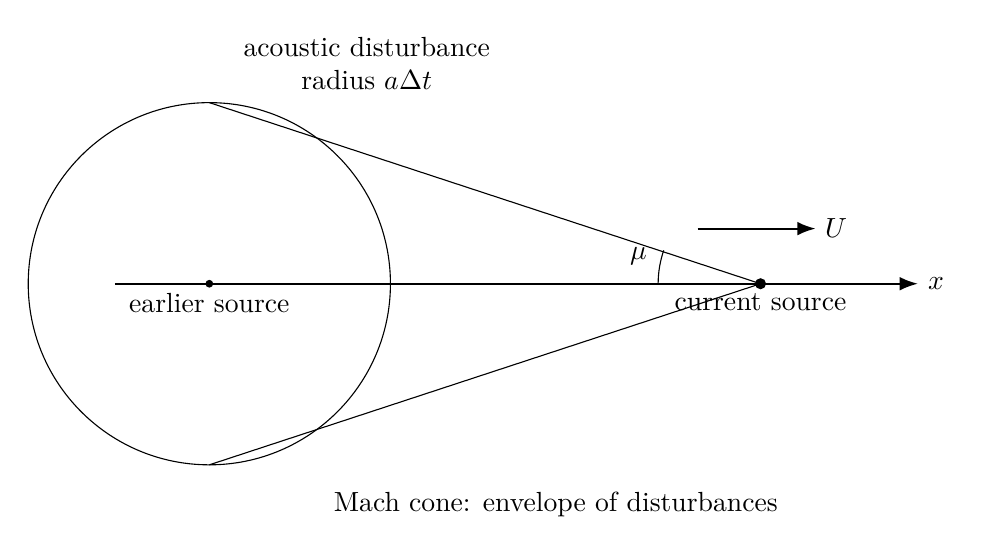
\begin{tikzpicture}[scale=1.0,>=Latex]
\draw[->,thick] (-0.2,0)--(10,0) node[right] {$x$};
\fill (1,0) circle(1.4pt) node[below] {earlier source};
\fill (8,0) circle(2pt) node[below] {current source};
\draw (1,0) circle(2.3);
\draw (8,0)--(1,2.3);
\draw (8,0)--(1,-2.3);
\draw[->,thick] (7.2,0.7)--(8.7,0.7) node[right] {$U$};
\draw (6.7,0) arc[start angle=180,end angle=161,radius=1.3];
\node at (6.45,.35) {$\mu$};
\node[align=center] at (3.0,2.8) {acoustic disturbance\\radius $a\Delta t$};
\node[align=center] at (5.4,-2.8) {Mach cone: envelope of disturbances};
\end{tikzpicture}
\end{center}

\textbf{Physical meaning.} Increasing $M$ narrows the cone. This changes where pressure disturbances intersect an off-body observation line and how signals from different parts of the vehicle interact.

\fromcfd{The clean Week 16 campaign fixes $M_\infty=1.8$. Later, the retained baseline and optimized geometries are recomputed at $M=1.7$ and $1.9$ to test whether the design improvement survives a modest change in operating condition.}
\checkpoint{Compute $\mu$ at $M=1.2$ and $M=3$. Which case has the wider region of upstream influence?}

\newpage
\topic{2}{Compression waves, shocks, and expansion fans}
A supersonic body turns the flow. Turning the flow into itself produces compression; turning it away produces expansion. The local slope distribution of the body therefore generates a train of compression and expansion disturbances.

\subtopic{2.1 Oblique compression and shock formation}
For a two-dimensional wedge or a locally inclined slender surface, the oblique-shock relation connects the upstream Mach number $M_1$, shock angle $\beta$, and flow deflection angle $\theta$:
\begin{equation}
\boxed{
\tan\theta=2\cot\beta\,
\frac{M_1^2\sin^2\beta-1}
{M_1^2(\gamma+\cos 2\beta)+2}.}
\end{equation}
The normal component is $M_{n1}=M_1\sin\beta$. Across the shock,
\begin{equation}
\boxed{\frac{p_2}{p_1}=1+\frac{2\gamma}{\gamma+1}\left(M_{n1}^2-1\right).}
\end{equation}
A weak compression wave travels slightly faster in its higher-pressure region. A sequence of compressions can therefore steepen and coalesce into a shock.

\subtopic{2.2 Prandtl--Meyer expansion}
A smooth convex turn produces a centered expansion fan. The Prandtl--Meyer function is
\begin{align}
\nu(M)=&\sqrt{\frac{\gamma+1}{\gamma-1}}
\tan^{-1}\sqrt{\frac{\gamma-1}{\gamma+1}(M^2-1)}\\
&-\tan^{-1}\sqrt{M^2-1}.
\end{align}
For an isentropic turn through angle $\theta$,
\begin{equation}
\boxed{\theta=\nu(M_2)-\nu(M_1).}
\end{equation}
Pressure falls through the fan while Mach number rises.

\subtopic{2.3 Why body shape matters}
A slender body's axial radius or area distribution controls where the local surface turns compress or expand the flow. Changing the distribution can split a strong compression into weaker events or shift wave interactions. Low-boom design is therefore not merely ``make the nose sharper'': the full longitudinal volume and lift distribution matters.

\begin{figure}[h]
\centering\includegraphics[width=.92\linewidth]{week16_generated/geometry_wave_concept.pdf}
\caption{Teaching-body profiles with conceptual supersonic wave directions. The dotted rays are pedagogical; the actual CFD solves the nonlinear Euler equations.}
\end{figure}

\checkpoint{Why can two bodies with the same total volume generate different off-body pressure signatures?}

\newpage
\topic{3}{From many waves to a sonic-boom signature}
\subtopic{3.1 Near-field and far-field waveforms}
Immediately around a vehicle, the pressure field contains multiple shocks and expansions associated with nose, volume changes, lift-producing surfaces, propulsion integration, and the tail. During propagation, nonlinear steepening, geometric spreading, and atmospheric absorption alter the signal. For a conventional configuration, multiple features may merge into an approximately N-shaped waveform with a rapid positive jump, gradual decay, a negative excursion, and a final recovery.

\begin{center}
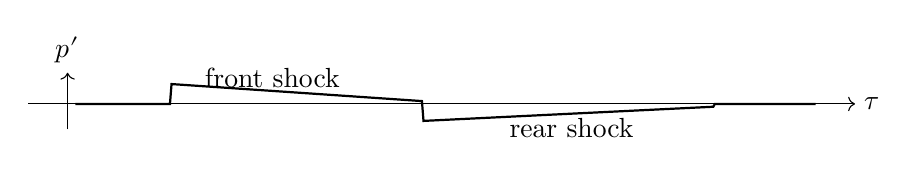
\begin{tikzpicture}[x=1cm,y=18cm]
\draw[->] (0,0)--(10.5,0) node[right] {$\tau$};
\draw[->] (.5,-.018)--(.5,.022) node[above] {$p'$};
\draw[thick] (.6,0)--(1.8,0)--(1.82,.014)--(5.0,.002)--(5.02,-.012)--(8.7,-.002)--(8.72,0)--(10,0);
\node[align=center] at (3.1,.018) {front shock};
\node[align=center] at (6.9,-.017) {rear shock};
\end{tikzpicture}
\end{center}

\subtopic{3.2 Equivalent area and the Whitham idea}
In classical slender-body sonic-boom theory, the aircraft is represented through an equivalent area distribution $A_e(x)$ that combines volume and, for lifting configurations, a lift-equivalent contribution. A commonly used Whitham-type transform has the form
\begin{equation}
F(y)\propto \int_0^y \frac{A_e''(x)}{\sqrt{y-x}}\,\dd x,
\end{equation}
with normalization depending on the chosen convention. The key lesson is that the pressure signature depends strongly on the \emph{second axial variation} of equivalent area, not merely on total volume. Smoothing or redistributing area changes where compression and expansion features appear.

\textbf{Why we do not use the $F$-function as the numerical solver here.} The Week 16 teaching case computes the nonlinear axisymmetric Euler field directly with SU2. The equivalent-area viewpoint is used to explain why shape redistribution can alter the pressure signature and why fixed volume is a meaningful design constraint.

\checkpoint{If two bodies have equal volume but different $A_e''(x)$, should they have identical boom signatures? Explain.}

\newpage
\topic{4}{What pressure quantity are we optimizing?}
CFD commonly reports the pressure coefficient
\begin{equation}
\boxed{C_p=\frac{p-p_\infty}{q_\infty}},\qquad q_\infty=\frac12\rho_\infty U_\infty^2.
\end{equation}
For a calorically perfect gas,
\begin{equation}
\rho_\infty U_\infty^2=\gamma p_\infty M_\infty^2,
\end{equation}
so pressure excess normalized by freestream static pressure is
\begin{equation}
\boxed{\frac{\Delta p}{p_\infty}=\frac{\gamma M_\infty^2}{2}C_p.}
\end{equation}
At $M_\infty=1.8$ and $\gamma=1.4$, the conversion factor is $2.268$. At $M=1.6$, it is $1.792$.

This conversion is essential when comparing sources: NASA sonic-boom records may use $\Delta p/p_\infty$, whereas the teaching-design plots use $C_p$.

\begin{figure}[h]
\centering\includegraphics[width=.92\linewidth]{week16_generated/representative_waveforms.pdf}
\caption{Representative accepted SU2 8.0.1 near-field pressure signatures from each data split. The waveform structure, not only the scalar peak, is important.}
\end{figure}

\fromcfd{The primary design objective is the maximum positive $C_p$ along the extraction line $r/L=0.5$. Pressure signatures are also extracted at $r/L=0.25$ and $0.75$ for diagnostic comparisons.}
\checkpoint{Convert $C_p=0.03$ to $\Delta p/p_\infty$ at $M=1.8$.}

\newpage
\topic{5}{Near-field shaping is not the same as ground loudness}
A complete sonic-boom prediction has at least three stages:
\begin{center}
\resizebox{.96\linewidth}{!}{%
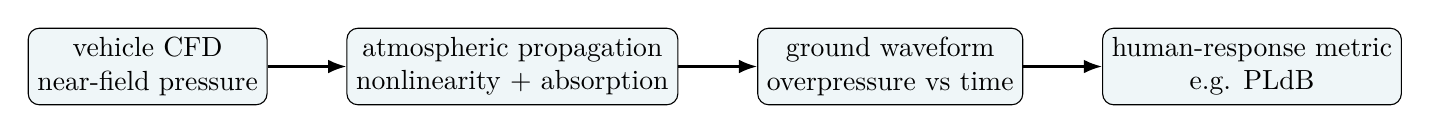
\begin{tikzpicture}[node distance=8mm and 10mm, every node/.style={draw,rounded corners,align=center,minimum height=9mm,fill=soft},>=Latex]
\node (cfd) {vehicle CFD\\near-field pressure};
\node[right=of cfd] (prop) {atmospheric propagation\\nonlinearity + absorption};
\node[right=of prop] (ground) {ground waveform\\overpressure vs time};
\node[right=of ground] (metric) {human-response metric\\e.g. PLdB};
\draw[->,thick] (cfd)--(prop);\draw[->,thick] (prop)--(ground);\draw[->,thick] (ground)--(metric);
\end{tikzpicture}}
\end{center}

\subtopic{5.1 Generalized Burgers-type propagation}
A schematic weak-shock propagation equation can be written as
\begin{equation}
\frac{\partial p'}{\partial s}
+\underbrace{\beta_n p'\frac{\partial p'}{\partial \tau}}_{\text{nonlinear steepening}}
=\underbrace{\delta\frac{\partial^2p'}{\partial\tau^2}}_{\text{thermoviscous absorption}}
+\underbrace{\mathcal{G}[p']}_{\text{geometric spreading}}
+\underbrace{\mathcal{A}[p']}_{\text{atmospheric effects}},
\end{equation}
where $s$ is propagation distance and $\tau$ is retarded time. Practical augmented Burgers solvers can also include molecular relaxation, humidity, temperature stratification, wind, and ray-tube geometry.

\subtopic{5.2 Why PLdB requires more than a peak}
Perceived loudness depends on the full time history and its frequency content. Two waveforms with the same maximum overpressure can have different rise times, durations, spectral distributions, and therefore different loudness. A smaller near-field $C_p$ peak is a useful design indicator, but it is not a PLdB calculation.

\warningbox{Week 16 stops before atmospheric propagation. The correct conclusion is ``verified reduction of a near-field pressure peak under the stated CFD model,'' not ``verified quieter sonic boom on the ground.''}

\newpage
\topic{6}{The teaching geometry: changing shape without shrinking the body}
Let $s=x/L$ and define an unnormalized radius function
\begin{equation}
f(s;a,b)=\sin(\pi s)\exp\!\left[a(2s-1)+b\cos(2\pi s)\right].
\end{equation}
The radius is
\begin{equation}
r(s)=c f(s;a,b).
\end{equation}
For a body of revolution,
\begin{equation}
V=\pi L\int_0^1 r(s)^2\,\dd s=\pi Lc^2\int_0^1 f(s)^2\,\dd s.
\end{equation}
Solving for $c$ gives
\begin{equation}
\boxed{c=\sqrt{\frac{V}{\pi L\int_0^1 f(s)^2\,\dd s}}.}
\end{equation}
Thus every $(a,b)$ pair has the same target volume. The teaching case uses $L=1\,\mathrm{m}$ and
\begin{equation}
V=\frac{\pi(0.06\,\mathrm{m})^2L}{2}.
\end{equation}

Parameter $a$ shifts volume fore or aft; parameter $b$ changes the balance between central and end regions. Fixed volume prevents a trivial optimizer from reducing pressure simply by making the body smaller.

\begin{figure}[h]
\centering\includegraphics[width=.92\linewidth]{week16_generated/geometry_profiles.pdf}
\caption{Three fixed-volume bodies. The retained optimized design is $a=0.32495$, $b=0.12238$.}
\end{figure}

\textbf{What this geometry is not.} It is not the Beihang TMS-10 aircraft, not a wing-body configuration, and not a complete transport vehicle. Cabin volume, structural thickness, lift, trim, propulsion, and viscous drag are outside this teaching model.
\checkpoint{Why is fixed volume necessary for a meaningful comparison? What additional constraints would a transport-aircraft design require?}

\newpage
\topic{7}{Governing equations used in the CFD}
\subtopic{7.1 Axisymmetric compressible Euler equations}
The computational mesh is two-dimensional in the meridional $(x,r)$ plane, but the physical body is three-dimensional and axisymmetric. A convenient weighted conservative form is
\begin{equation}
\boxed{
\frac{\partial(r\vect U)}{\partial t}
+\frac{\partial(r\vect F)}{\partial x}
+\frac{\partial(r\vect G)}{\partial r}
=\vect S,}
\end{equation}
with
\begin{equation}
\vect U=\begin{bmatrix}\rho\\ \rho u\\ \rho v\\ \rho E\end{bmatrix},\quad
\vect F=\begin{bmatrix}\rho u\\ \rho u^2+p\\ \rho uv\\ (\rho E+p)u\end{bmatrix},\quad
\vect G=\begin{bmatrix}\rho v\\ \rho uv\\ \rho v^2+p\\ (\rho E+p)v\end{bmatrix},
\end{equation}
and the axisymmetric geometric source
\begin{equation}
\vect S=\begin{bmatrix}0\\0\\p\\0\end{bmatrix}.
\end{equation}
The pressure is recovered from total energy using the perfect-gas relation
\begin{equation}
\boxed{p=(\gamma-1)\left[\rho E-\frac{\rho(u^2+v^2)}{2}\right].}
\end{equation}

\textbf{Why the radial source matters.} A planar two-dimensional Euler calculation omits the geometric divergence of an axisymmetric flow. Treating the meridional outline as an ordinary 2-D airfoil would therefore solve a different physical problem.

\subtopic{7.2 Pressure drag}
For an axisymmetric body with radius $r(x)$, the axial pressure force can be written
\begin{equation}
D_p=2\pi\int_0^L (p-p_\infty)\,r\frac{\dd r}{\dd x}\,\dd x,
\end{equation}
with sign determined by the surface orientation convention. The nondimensional teaching metric is
\begin{equation}
\boxed{C_{D,p}=\frac{D_p}{q_\infty L^2}.}
\end{equation}
This is pressure drag only. Skin friction is absent because the Euler equations are inviscid.

\fromcfd{The design objective minimizes the maximum $C_p$ at $r/L=0.5$ subject to $C_{D,p}\le1.02C_{D,p,0}$ and the exact fixed-volume parameterization.}

\newpage
\topic{8}{What we actually ran: CFD setup and acceptance gates}
\subtopic{8.1 Physical and numerical setup}
The accepted clean campaign uses Gmsh meshes and the checksum-pinned official SU2 8.0.1 solver. The freestream and geometry are deliberately simple so that every design can be recomputed and audited.

\begin{center}
\begin{tabular}{ll}
\toprule
Quantity & Teaching value\\\midrule
Geometry & axisymmetric body of revolution, zero incidence\\
Length & $L=1\,\mathrm{m}$\\
Freestream Mach & $M_\infty=1.8$\\
Freestream pressure & $p_\infty=101325\,\mathrm{Pa}$\\
Freestream temperature & $T_\infty=288.15\,\mathrm{K}$\\
Governing model & compressible Euler, ideal gas\\
Primary extraction line & $r/L=0.5$\\
Other extraction lines & $r/L=0.25$ and $0.75$\\
Reference area for $C_{D,p}$ & $L^2$\\
Training mesh level & 1.5\\
Typical design cells & 45,408 (level 1.5), 80,640 (level 2)\\
\bottomrule
\end{tabular}
\end{center}

\subtopic{8.2 Why a residual is not enough}
Every accepted label must pass numerical and full-field physical rejection gates. The clean campaign requires finite positive pressure and density, final log$_{10}$ density residual no larger than $-9$, at least five orders of residual reduction, pressure-drag variation below $10^{-4}$ over the final 100 iterations, maximum total-enthalpy deviation no larger than 10\%, and density below 110\% of the isentropic stagnation bound. These thresholds are rejection criteria, not estimates of physical uncertainty.

\subtopic{8.3 Accepted CFD field evidence}
\begin{figure}[h]
\centering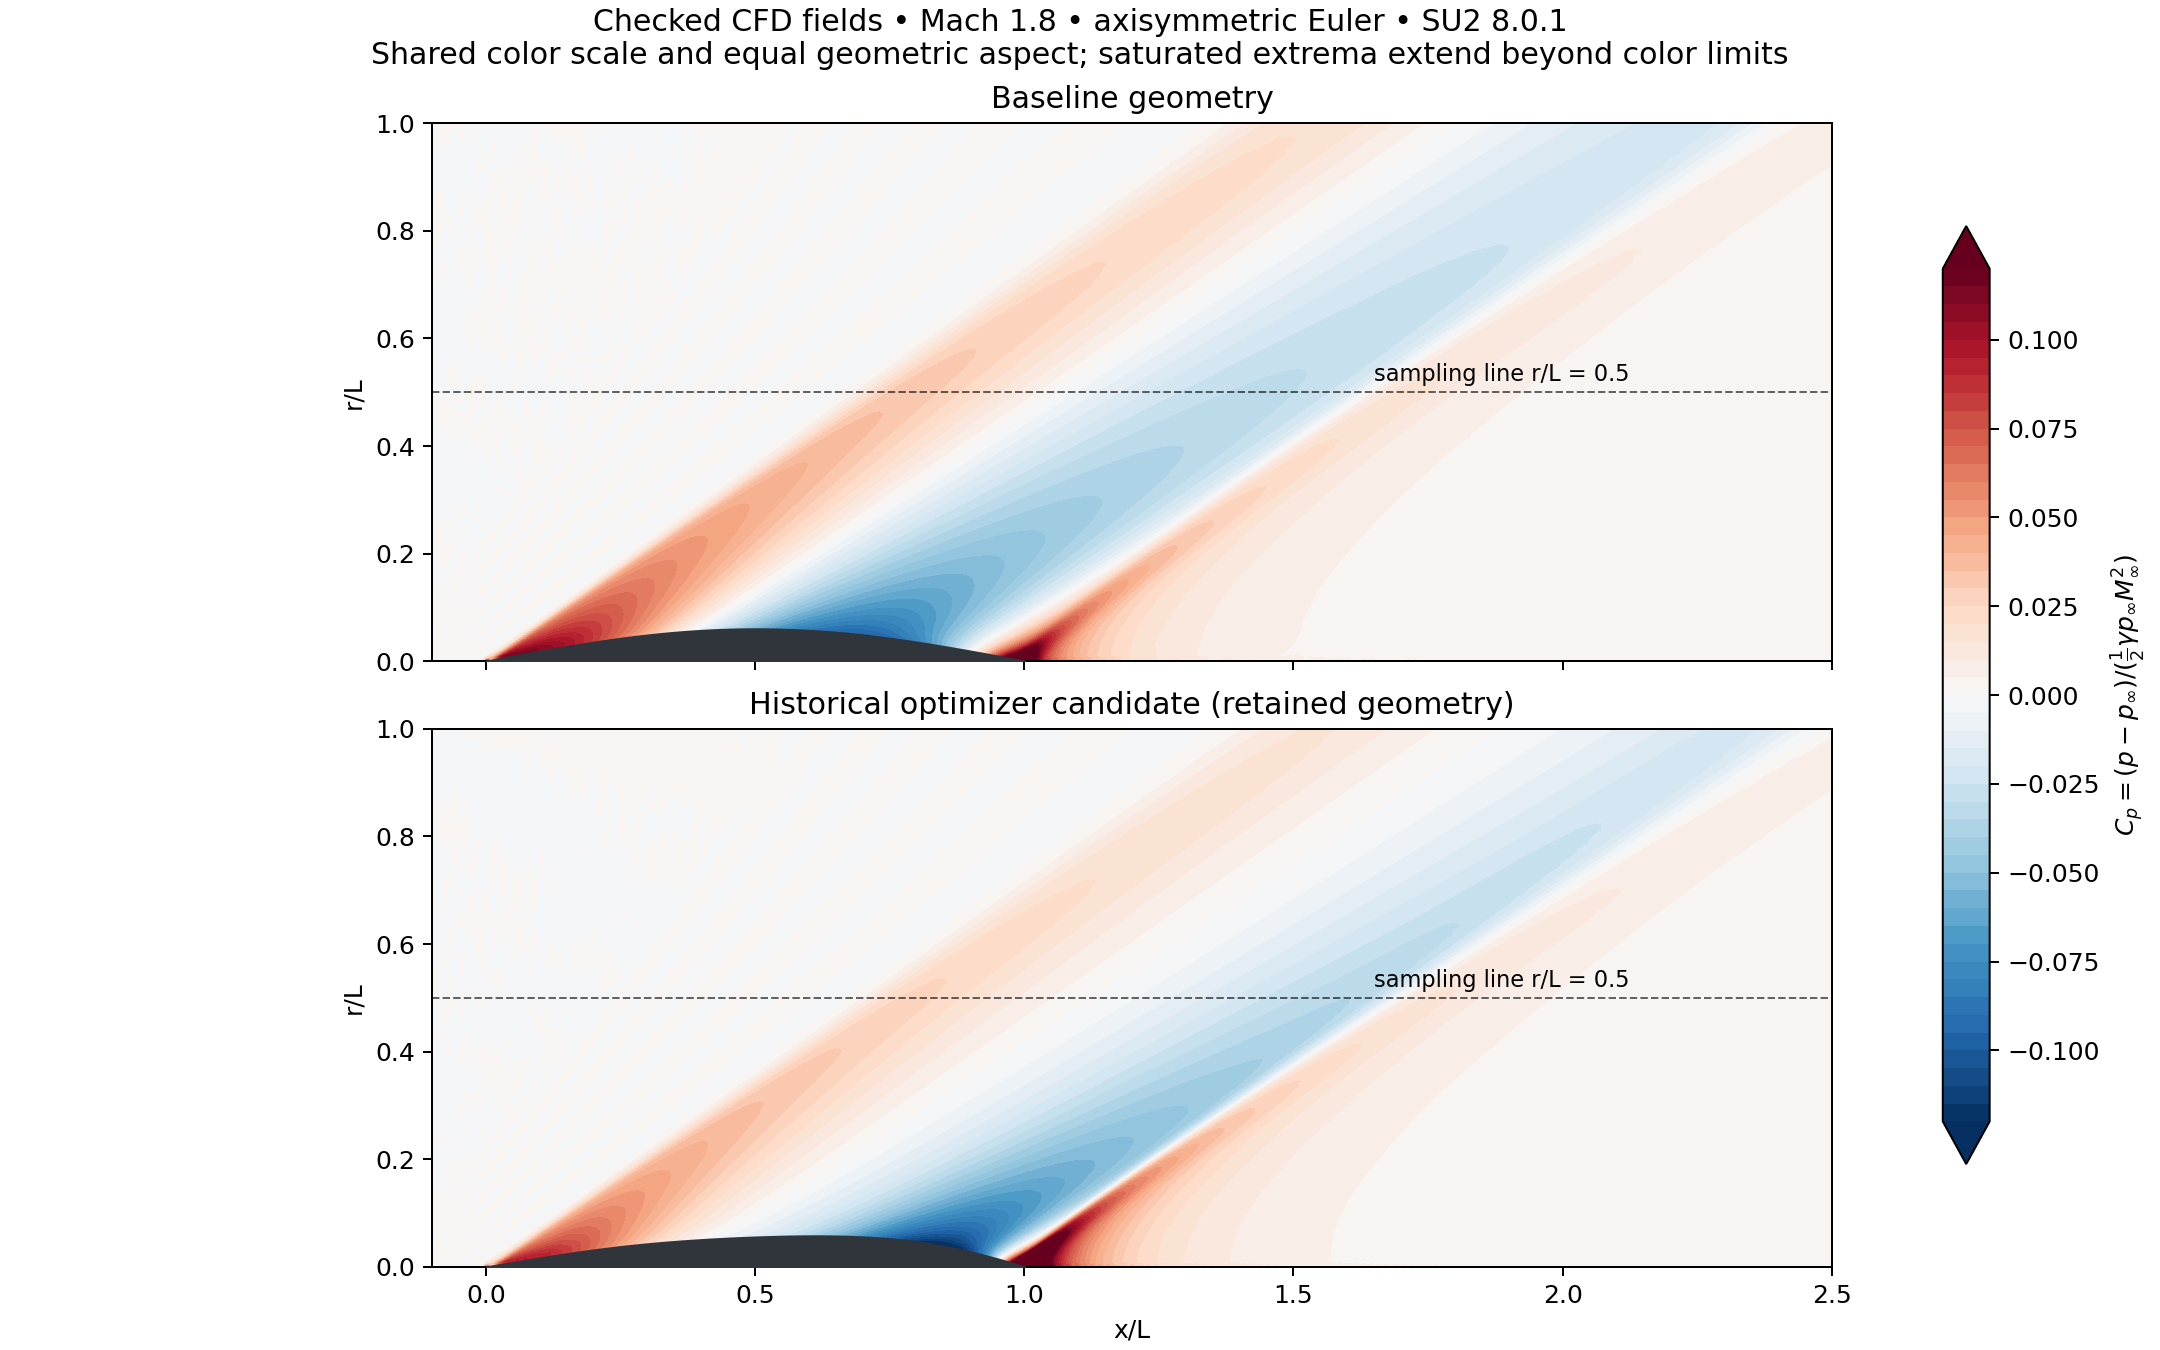
\includegraphics[width=.98\linewidth]{../../results/week16_lowboom/reference/clean_cfd_fields.png}
\caption{Accepted SU2 8.0.1 fields for the teaching body. The field plots are part of the retained physical/numerical evidence, not decorative illustrations.}
\end{figure}

\checkpoint{A run reaches a density residual of $10^{-11}$ but has a large local total-enthalpy defect near the tip. Should it be accepted? Why not?}

\newpage
\topic{9}{Verification before machine learning}
\textbf{Verification asks: are we solving the chosen equations correctly?} It is different from validation, which asks whether the model agrees with reality for the intended quantity.

\subtopic{9.1 Taylor--Maccoll cone benchmark}
Supersonic flow over a cone admits an axisymmetric similarity solution. The Taylor--Maccoll ODE system is integrated from an attached conical shock to the cone surface. The shock angle is adjusted until the polar velocity satisfies the wall-tangency condition. This provides an independent pressure reference that does not use SU2's finite-volume discretization.

For a 7-degree cone at $M=1.8$, the retained mesh study uses 24,000, 96,000, and 216,000 fluid cells. The wall-$C_p$ errors relative to the independent Taylor--Maccoll solution are 4.563\%, 2.156\%, and 1.162\%. The last-two mean-$C_p$ change is 1.006\%.

\begin{figure}[h]
\centering\includegraphics[width=.72\linewidth]{week16_generated/cone_refinement.pdf}
\caption{Taylor--Maccoll wall-pressure error decreases with refinement. The coarse pressure criterion fails, while the declared refined-family verification criteria pass.}
\end{figure}

\begin{center}
\begin{tabular}{rrrr}
\toprule
Fluid cells & CFD mean $C_p$ & error to Taylor--Maccoll & numerical/physical gates\\\midrule
24,000 & 0.059175 & 4.563\% & pass\\
96,000 & 0.060667 & 2.156\% & pass\\
216,000 & 0.061284 & 1.162\% & pass\\
\bottomrule
\end{tabular}
\end{center}

\textbf{Interpretation.} The cone verifies a specific component of the solver/model chain: axisymmetric inviscid supersonic wall pressure. It does not experimentally validate the boom waveform, the teaching geometry, or the neural network.

\newpage
\topic{10}{The 44-case dataset and the reduced-order learning problem}
\subtopic{10.1 Frozen data split}
The clean SU2 8.0.1 campaign contains 44 geometries: 24 training, 6 validation, 8 test, and 6 extrapolation cases. All belong to the same two-parameter family. The extrapolation cases extend one shape parameter beyond the training region; they do not introduce a new topology.

\begin{figure}[h]
\centering\includegraphics[width=.72\linewidth]{week16_generated/split_map.pdf}
\caption{Frozen geometry split. Training statistics, scalers, and POD modes must be fitted only on the training subset.}
\end{figure}

\subtopic{10.2 Proper Orthogonal Decomposition}
Let each CFD signature be a row vector $\vect y_i=[C_p(x_1),\ldots,C_p(x_m)]$. Form the training matrix $Y$ and subtract the training mean:
\begin{equation}
Y'=Y-\overline{Y}.
\end{equation}
The singular value decomposition is
\begin{equation}
\boxed{Y'=U\Sigma V^T.}
\end{equation}
The first $K$ rows of $V^T$ are POD modes $\phi_k(x)$. A waveform is reconstructed as
\begin{equation}
\boxed{C_p(x;\theta)\approx \overline C_p(x)+\sum_{k=1}^{K}z_k(\theta)\phi_k(x).}
\end{equation}
The retained model uses $K=12$ full-SVD modes. The retained energy is
\begin{equation}
E_K=\frac{\sum_{k=1}^K\sigma_k^2}{\sum_j\sigma_j^2}.
\end{equation}

\begin{figure}[h]
\centering\includegraphics[width=.72\linewidth]{week16_generated/pod_energy.pdf}
\caption{Cumulative POD energy of the 24 training waveforms. Compression reduces a 561-point CFD signature to a small set of modal coefficients.}
\end{figure}

\newpage
\topic{11}{Neural surrogate: what is learned, and how do we judge it?}
The retained clean model maps two geometry parameters to 12 POD coefficients and log pressure drag:
\begin{equation}
(a,b)\longrightarrow [z_1,\ldots,z_{12},\log C_{D,p}].
\end{equation}
Its architecture is a 32--32 tanh MLP trained with L-BFGS, $\alpha=0.01$, random seed 16, and training-only scaling. The full-SVD POD basis is also fitted only on the 24 training cases.

\subtopic{11.1 Three error measures}
Whole-waveform relative error:
\begin{equation}
\epsilon_{\rm wave}=\frac{\|\widehat{\vect y}-\vect y\|_2}{\|\vect y\|_2}.
\end{equation}
Mean positive-peak relative error:
\begin{equation}
\epsilon_{\rm peak}=\left|\frac{\max \widehat C_p-\max C_p}{\max C_p}\right|.
\end{equation}
Pressure-drag relative error:
\begin{equation}
\epsilon_D=\left|\frac{\widehat C_{D,p}-C_{D,p}}{C_{D,p}}\right|.
\end{equation}
A shock can be shifted in $x$ while retaining a similar peak amplitude; therefore peak error alone can hide a poor waveform.

\begin{figure}[h]
\centering\includegraphics[width=.82\linewidth]{week16_generated/model_errors.pdf}
\caption{Clean-model errors across the frozen splits. Extrapolation is substantially harder than interpolation. A log scale is used so that training and extrapolation errors remain visible together.}
\end{figure}

\begin{center}\small
\begin{tabular}{lrrrr}
\toprule
Split & wave $L_2$ & mean peak & mean drag & worst waveform\\\midrule
Train (24) & 0.313\% & 0.189\% & 0.112\% & 0.648\%\\
Validation (6) & 3.935\% & 1.602\% & 2.254\% & 6.343\%\\
Test (8) & 5.369\% & 1.406\% & 2.559\% & 11.775\%\\
Extrapolation (6) & 34.286\% & 6.831\% & 22.389\% & 43.190\%\\
Finer CFD test (8) & 7.204\% & 2.237\% & 2.274\% & 15.372\%\\
\bottomrule
\end{tabular}
\end{center}

\textbf{Lesson.} Aggregate criteria can pass while one geometry has a much larger error. Report the worst individual case, and do not claim reliable extrapolation from good interpolation results.

\newpage
\topic{12}{Optimization: let the surrogate propose, let CFD decide}
The constrained design problem is
\begin{equation}
\boxed{\min_{a,b}\; \max_x C_p(x,r/L=0.5;a,b)}
\end{equation}
subject to
\begin{equation}
\boxed{C_{D,p}(a,b)\le1.02C_{D,p,0}},
\end{equation}
and the exact fixed-volume parameterization of Section 6.

A learned surrogate makes a large number of candidate evaluations cheap, but this creates a new danger: an optimizer actively searches for regions where surrogate error can be exploited. Ordinary test-set accuracy is therefore not enough. The proposed optimum must be meshed again and solved with CFD.

\subtopic{12.1 Retained design}
The retained candidate has
\begin{equation}
a=0.3249533,\qquad b=0.1223779.
\end{equation}
At mesh level 1.5, the baseline and optimized bodies use 45,408 fluid cells. At level 2 they use 80,640 cells.

\begin{center}\small
\begin{tabular}{lrrrr}
\toprule
Case & peak $C_p$ & $C_{D,p}$ & peak change & drag change\\\midrule
Baseline, level 1.5 & 0.0333075 & 0.00135423 & -- & --\\
Optimized, level 1.5 & 0.0262504 & 0.00130281 & $-21.188\%$ & $-3.797\%$\\
Baseline, level 2 & 0.0341276 & 0.00136763 & -- & --\\
Optimized, level 2 & 0.0270753 & 0.00131947 & $-20.665\%$ & $-3.522\%$\\
\bottomrule
\end{tabular}
\end{center}

\begin{figure}[h]
\centering\includegraphics[width=.92\linewidth]{week16_generated/design_waveforms.pdf}
\caption{Fresh SU2 8.0.1 recomputation of baseline and retained optimized signatures on two mesh levels. The improvement is measured from CFD, not accepted from the neural prediction.}
\end{figure}

\subtopic{12.2 Mesh sensitivity}
For the baseline, the level-1.5 to level-2 changes are 2.403\% in peak, 0.980\% in pressure drag, and 3.586\% in the waveform $L_2$ measure. For the optimized body they are 3.047\%, 1.262\%, and 5.395\%. The declared peak and drag gates pass. The waveform difference is reported separately rather than hidden behind scalar agreement.

\checkpoint{Why is a fresh CFD solve of the optimized geometry more important than a very small training error?}

\newpage
\topic{13}{Off-design behavior and robustness}
The surrogate was trained at $M=1.8$. To test the retained geometry rather than the learned model, the baseline and optimized bodies were recomputed directly with SU2 at $M=1.7$ and $1.9$.

\begin{center}
\begin{tabular}{lrr}
\toprule
Mach & peak-pressure reduction & pressure-drag reduction\\\midrule
1.7 & 21.010\% & 3.231\%\\
1.8 & 21.188\% & 3.797\%\\
1.9 & 21.166\% & 4.311\%\\
\bottomrule
\end{tabular}
\end{center}

\begin{figure}[h]
\centering\includegraphics[width=.72\linewidth]{week16_generated/offdesign.pdf}
\caption{Direct CFD off-design evidence. These points are not neural-network predictions.}
\end{figure}

\textbf{What this establishes.} The local design benefit survives two nearby Mach-number perturbations for the teaching geometry and the chosen metrics. It does not establish a complete flight envelope, uncertainty quantification, or robustness to altitude, angle of attack, Reynolds number, atmospheric state, or manufacturing variation.

\newpage
\topic{14}{NASA SEEB-ALR: a useful failed research extension}
The NASA SEEB-ALR benchmark is separate from the two-parameter teaching body. It provides an as-built geometry and off-body wind-tunnel records at $M=1.6$, making it attractive for experimental validation of a CFD chain.

\subtopic{14.1 Pressure convention and geometry alignment}
The NASA pressure ordinate is $\Delta p/p_\infty$, not $C_p$. At $M=1.6$ and $\gamma=1.4$, use
\begin{equation}
\frac{\Delta p}{p_\infty}=1.792\,C_p.
\end{equation}
The retained source macros prescribe longitudinal shifts; no fitted shock-position shift should be introduced merely to reduce error. The original finite nose and downstream sting must be retained.

\begin{figure}[h]
\centering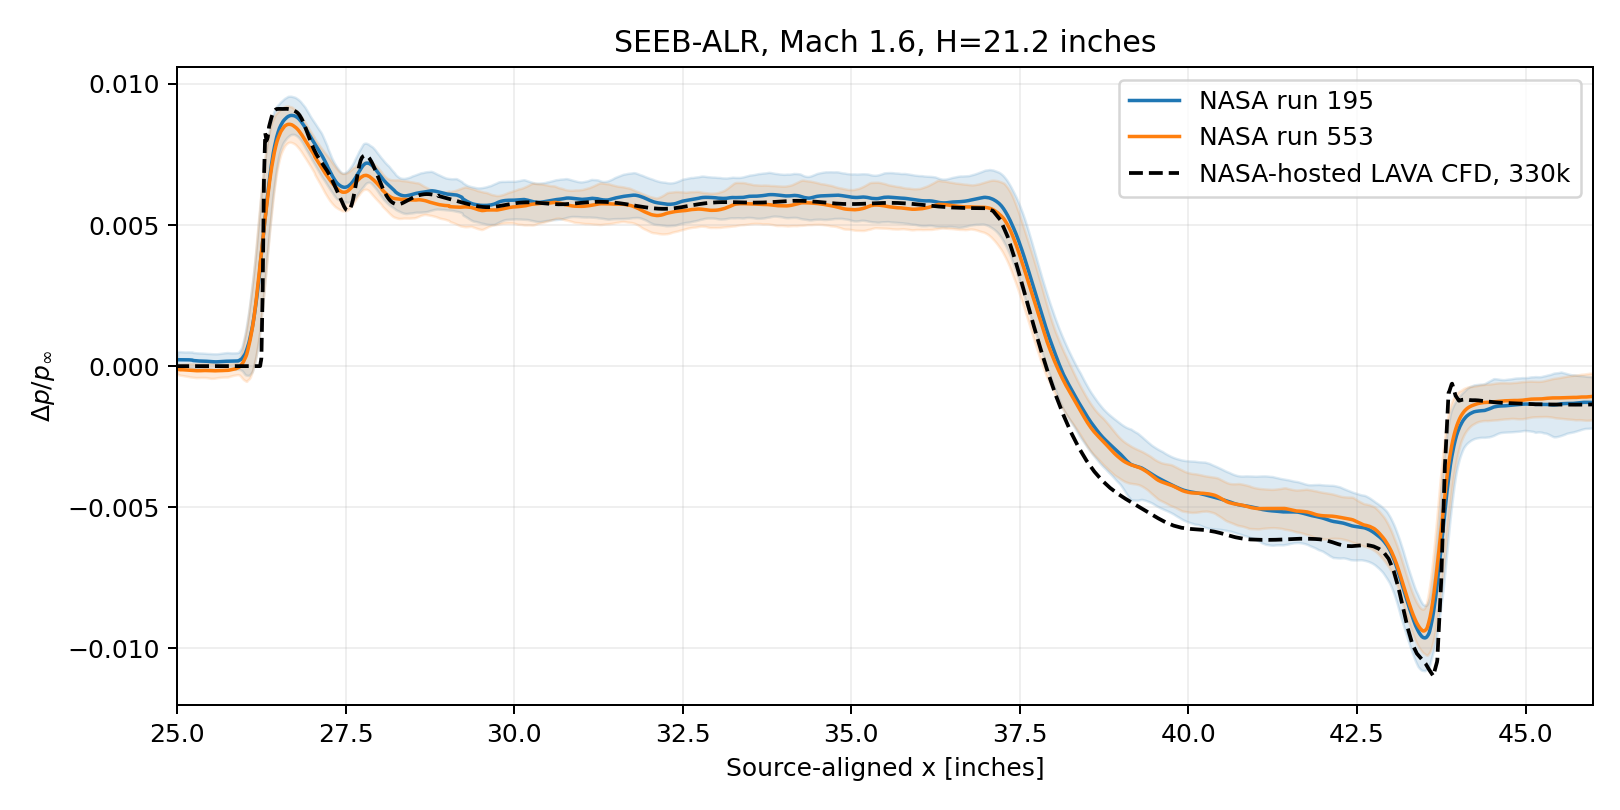
\includegraphics[width=.92\linewidth]{../../results/week16_lowboom/reference/seeb_comparison.png}
\caption{Retained NASA-hosted LAVA CFD compared with two NASA wind-tunnel records. This is a reference comparison, not a successful SU2 validation by this project.}
\end{figure}

For the fixed 25--46 inch comparison window, the retained LAVA-to-experiment waveform errors are 14.75\% and 15.02\%, with peak errors 2.64\% and 6.41\% for NASA runs 195 and 553, respectively.

\subtopic{14.2 Why our attempted SU2 reproduction was rejected}
The NASA recovery runs did not establish an accepted physically checked, mesh-refined family. Earlier nose treatment produced unphysical stagnation behavior. Later replays still failed convergence/physical gates. The correct scientific action is to preserve the failure, document it, and exclude it from the accepted release claims.

\warningbox{A solver exit code, a visually plausible pressure curve, or a small residual cannot turn an unaccepted NASA run into validation evidence. The Week 16 release therefore reports NASA as a deferred failed research extension.}

\newpage
\topic{15}{Verification, validation, and ML validation are different}
\begin{center}
\begin{tabular}{p{.22\linewidth}p{.32\linewidth}p{.36\linewidth}}
\toprule
Question & Typical evidence & Week 16 example\\\midrule
Numerical verification & residuals, mesh refinement, analytical benchmark, conservation/physical checks & Taylor--Maccoll cone; design mesh sensitivity; full-field gates\\
Physical validation & comparison with suitable experiment and uncertainty & NASA SEEB-ALR is a target, but the SU2 reproduction is not accepted\\
ML validation & frozen data splits, train-only preprocessing, held-out CFD, worst-case errors & clean 24/6/8/6 split; finer-CFD comparison; extrapolation stress test\\
Design verification & fresh high-fidelity recomputation of the proposed optimum & baseline/optimized SU2 8.0.1 recomputation on two meshes\\
\bottomrule
\end{tabular}
\end{center}

\textbf{The central logical chain is}
\begin{equation*}
\boxed{\text{physics}\rightarrow\text{verified CFD}\rightarrow\text{reduced model}\rightarrow\text{surrogate proposal}\rightarrow\text{fresh CFD check}.}
\end{equation*}
The neural model accelerates the search; it does not replace verification.

\subtopic{15.1 What we actually completed}
\begin{center}\small
\begin{longtable}{p{.40\linewidth}p{.16\linewidth}p{.32\linewidth}}
\toprule
Computational campaign & Outcome & Retained evidence\\\midrule
44-case clean-label SU2 8.0.1 campaign & PASS & 24 train / 6 validation / 8 test / 6 extrapolation; all declared full-field gates pass\\
Fixed clean-label MLP audit & PASS & same-mesh and finer-mesh metrics retained; extrapolation failure reported\\
Taylor--Maccoll three-mesh refinement & PASS & finest wall-$C_p$ error 1.162\%; last-two change 1.006\%\\
Retained optimized-design recomputation & PASS & peak reduction 21.188\% and 20.665\% on two meshes; drag constraint passes\\
Off-design $M=1.7,1.9$ recomputation & PASS & near-field peak reduction remains about 21\%\\
NASA SEEB-ALR SU2 reproduction & FAIL / deferred & failure retained; excluded from accepted validation claims\\
\bottomrule
\end{longtable}
\end{center}

\textbf{GitHub Actions provenance for the accepted scientific runs.} Clean campaign run 35944299803; clean model run 35944888983; retained-design verification run 35943668623; Taylor--Maccoll refinement run 35943668572; verified publication candidate run 36002078532. NASA recovery/replay runs 35944409924 and 35946027208 failed and remain deferred.

\newpage
\topic{16}{Student interpretation and exercises}
\textbf{Exercise 1: Mach geometry.} Compute $\mu$ for $M=1.4,1.6,2.0,2.5$. Explain why the cone narrows as Mach increases.

\textbf{Exercise 2: pressure normalization.} At $M=1.8$, convert $C_p=0.03$ to $\Delta p/p_\infty$. Repeat at $M=1.6$.

\textbf{Exercise 3: fixed volume.} Choose two new $(a,b)$ pairs, evaluate $r(s)$ numerically, and verify the target volume to better than $10^{-5}$ relative error.

\textbf{Exercise 4: POD truncation.} Repeat the learning problem with $K=4,8,12$. Compare retained energy and test waveform error.

\textbf{Exercise 5: data leakage.} Intentionally fit the POD basis on all 44 cases. Why might the apparent test error improve, and why is that result scientifically invalid?

\textbf{Exercise 6: shock location versus peak.} Find the test case with the largest waveform $L_2$ error. Determine whether the dominant error is amplitude, shock position, or both.

\textbf{Exercise 7: tighter constraint.} Replace the drag limit $1.02C_{D,p,0}$ with $1.00C_{D,p,0}$. How does the feasible design region change?

\textbf{Exercise 8: claim discipline.} Write one sentence that is justified by the Week 16 evidence and one sentence that would be an overclaim. Your justified sentence must distinguish near-field pressure from ground loudness.

\checkpoint{If the optimized near-field peak falls 21\% but the atmospheric propagation model is never run, what is the strongest defensible statement?}

\topic{17}{Take-away}
The most important result of Week 16 is not a particular pair $(a,b)$. It is a defensible computational workflow:
\begin{enumerate}
\item start from compressible-flow physics and meaningful constraints;
\item solve a clearly stated CFD model;
\item verify the solver/model chain with independent numerical evidence;
\item generate a frozen training/validation/test dataset;
\item compress the waveform with training-only POD;
\item use a surrogate to explore designs cheaply;
\item recompute the proposed design with CFD;
\item report mesh sensitivity, worst-case ML errors, off-design checks, and failed extensions;
\item stop the scientific claim at the boundary of the evidence.
\end{enumerate}

For the retained teaching body, the optimized geometry reduces the verified near-field peak by about 21\% while also reducing pressure drag on two meshes. The clean neural surrogate is accurate for interpolation within the two-parameter family but degrades strongly under extrapolation. NASA experimental CFD validation remains unresolved. Ground sonic-boom loudness remains outside the computed scope.

\newpage
\section*{References}
\addcontentsline{toc}{section}{References}
Zheng, Q., Liang, Y., Yang, Y. and Pan, C. (2026). ``Research on low-drag low-boom supersonic transport configuration using an MDO framework and deep learning methods.'' \emph{Aerospace Science and Technology}, 178, 113218. DOI: 10.1016/j.ast.2026.113218.

Taylor, G. I. and Maccoll, J. W. (1933). ``The air pressure on a cone moving at high speeds.'' \emph{Proceedings of the Royal Society A}, 139, 278--297.

SU2 project documentation and governing-equation references: \url{https://su2code.github.io/}. The accepted Week 16 clean campaign uses the checksum-pinned official SU2 8.0.1 executable.

Gmsh reference manual: \url{https://gmsh.info/doc/texinfo/gmsh.html}.

AIAA/NASA Sonic Boom Prediction Workshop material: \url{https://lbpw.larc.nasa.gov/}. NASA SEEB-ALR source data and original coordinate macros are retained in the Week 16 reference directory with provenance records.

FlowMLLab Week 16 evidence is retained under the repository paths \path{results/week16_lowboom/}, \path{notebooks/week16/}, and \path{cases/week16_lowboom/}. The model and NASA validation guides are in the Week 16 notebook directory.

\end{document}
